% !TEX root = main.tex

%%%-------------------------------------------
\section{Алгоритм обратного распространения ошибки (Backpropagation)}

\epigraph{Что происходит, когда мы суём пальцы в розетку? Нас бьёт током! Мы делаем ошибку, и она распространяется по нашему телу назад.}{Твоя мама}


%%%-------------------------------------------
\begin{problem}{(граф вычислений)}
    Маша вспомнила картину из кофейни Добродума и решила нарисовать у себя дома свою такую же. Она хочет изобразить для функции  
    
    $$
    f(x,y) = x^2 + xy + (x + y)^2
    $$ 
    
    граф вычислений. В кругляшах она будет записывать результаты вычислений. Каждое ребро будет обозначать элементарную операцию: плюс или умножить.
    
    Когда картина будет нарисована, Маша хочет найти производные всех выходов из кругляшей по всем входам. Опираясь на получившийся граф Маша хочет выписать частные производные функции $f$ по $x$ и по $y$\footnote{По мотивам книги Николенко "Глубокое обучение" (стр. 79)}.
\end{problem} 


%%%-------------------------------------------
\begin{problem}{(придумываем backpropagation)}
	
Маша умеет собирать нейросети. Например, у неё есть такая нейросеть: 
	
\begin{center}
	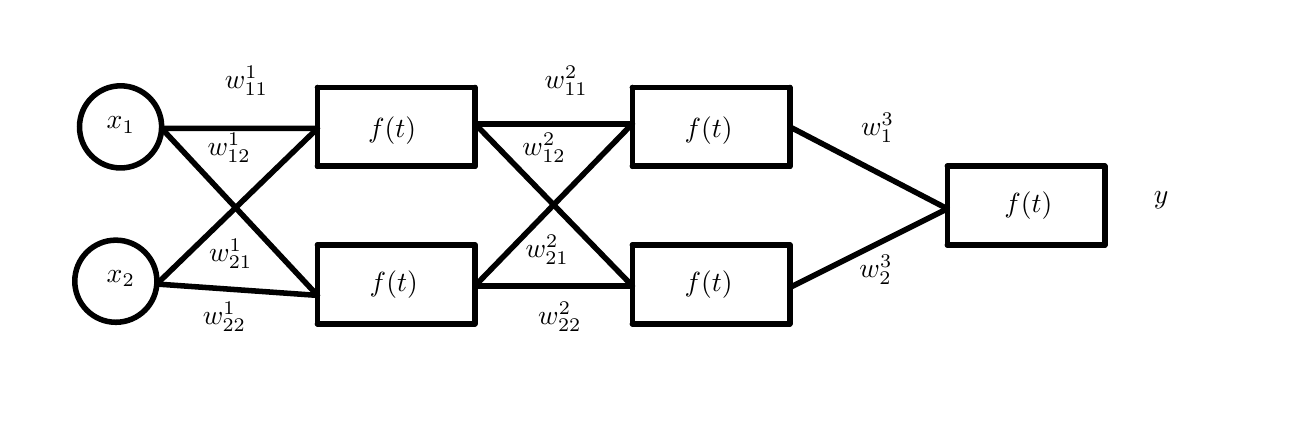
\begin{tikzpicture}[line cap=round,line join=roundx=1.0cm,y=1.0cm]
	\clip(-3.68,0.12) rectangle (12.02,4.76);
	\draw [line width=2.pt] (-2.56,1.54) circle (0.5215361924162121cm);
	\draw [line width=2.pt] (-2.5,3.5) circle (0.5215361924162117cm);
	\draw [line width=2.pt] (0.,4.)-- (2.,4.);
	\draw [line width=2.pt] (2.,4.)-- (2.,3.);
	\draw [line width=2.pt] (2.,3.)-- (0.,3.);
	\draw [line width=2.pt] (0.,3.)-- (0.,4.);
	\draw [line width=2.pt] (0.,2.)-- (2.,2.);
	\draw [line width=2.pt] (2.,2.)-- (2.,1.);
	\draw [line width=2.pt] (2.,1.)-- (0.,1.);
	\draw [line width=2.pt] (0.,1.)-- (0.,2.);
	\draw [line width=2.pt] (4.,4.)-- (6.,4.);
	\draw [line width=2.pt] (6.,4.)-- (6.,3.);
	\draw [line width=2.pt] (6.,3.)-- (4.,3.);
	\draw [line width=2.pt] (4.,3.)-- (4.,4.);
	\draw [line width=2.pt] (4.,2.)-- (6.,2.);
	\draw [line width=2.pt] (6.,2.)-- (6.,1.);
	\draw [line width=2.pt] (6.,1.)-- (4.,1.);
	\draw [line width=2.pt] (4.,1.)-- (4.,2.);
	\draw [line width=2.pt] (8.,3.)-- (10.,3.);
	\draw [line width=2.pt] (10.,3.)-- (10.,2.);
	\draw [line width=2.pt] (10.,2.)-- (8.,2.);
	\draw [line width=2.pt] (8.,2.)-- (8.,3.);
	\draw [line width=2.pt] (-1.9787961021013818,3.4813855750750493)-- (0.,3.48);
	\draw [line width=2.pt] (-1.9787961021013818,3.4813855750750493)-- (0.,1.36);
	\draw [line width=2.pt] (-2.039699677075342,1.5041172191086443)-- (0.,1.36);
	\draw [line width=2.pt] (-2.039699677075342,1.5041172191086443)-- (0.,3.48);
	\draw [line width=2.pt] (2.,3.54)-- (4.,3.54);
	\draw [line width=2.pt] (2.,1.48)-- (4.,1.48);
	\draw [line width=2.pt] (2.,1.48)-- (4.,3.54);
	\draw [line width=2.pt] (2.,3.54)-- (4.,1.48);
	\draw [line width=2.pt] (6.,3.5)-- (8.,2.46);
	\draw [line width=2.pt] (6.,1.46)-- (8.,2.46);
	\draw (4.54, 3.75) node[anchor=north west] {$f(t)$};
	\draw (4.54,1.8) node[anchor=north west] {$f(t)$};
	\draw (0.52, 3.75) node[anchor=north west] {$f(t)$};
	\draw (0.54, 1.8) node[anchor=north west] {$f(t)$};
	\draw (8.6, 2.8) node[anchor=north west] {$f(t)$};
	\draw (-2.8, 1.8) node[anchor=north west] {$x_2$};
	\draw (-2.8, 3.75) node[anchor=north west] {$x_1$};
	\draw (6.78,3.8) node[anchor=north west] {$w_1^3$};
	\draw (6.76,2) node[anchor=north west] {$w_{2}^3$};
	\draw (-1.3,4.4) node[anchor=north west] {$w_{11}^1$};
	\draw (-1.5,2.2) node[anchor=north west] {$w_{21}^1$};
	\draw (-1.52,3.55) node[anchor=north west] {$w_{12}^1$};
	\draw (-1.58,1.4) node[anchor=north west] {$w_{22}^1$};
	\draw (2.76,4.4) node[anchor=north west] {$w_{11}^2$};
	\draw (2.68,1.4) node[anchor=north west] {$w_{22}^2$};
	\draw (2.52,2.25) node[anchor=north west] {$w_{21}^2$};
	\draw (2.48,3.55) node[anchor=north west] {$w_{12}^2$};
	\draw (10.5, 2.8) node[anchor=north west] {$y$};
	\end{tikzpicture}
\end{center}	

Здесь $w_{ij}^k$ --- веса для $k$ слоя, $f(t)$ --- какая-то функция активации. Маша хочет научиться делать для такой нейронной сетки градиентный спуск: 

\begin{enumerate}
	\item  Запишите Машину нейросеть как сложную функцию. Сначала в обычной записи, а затем в матричном виде. 
	
	\item  Пусть $L(W_1, W_2, W_3) = \frac{1}{2} \cdot (y - \hat y)^2$ --- функция потерь, где $W_k$ --- веса $k-$го слоя.  Найдите производные функции $L$ по всем весам $W_k$.
	
	\item В производных постоянно повторяются одни и те же части. Постоянно искать их не очень оптимально. Выделите эти часть в прямоугольнички цветными ручками. 
	
	\item Выпишите все производные в том виде, в котором их было бы удобно использовать для алгоритма обратного распространения ошибки, а затем, сформулируйте сам алгоритм.
\end{enumerate}
\end{problem}


%%%-------------------------------------------
\begin{problem}{(backpropagation руками)}

    Маша как-то раз решала задачу классифкации. С тех пор у неё в кармане завалялась нейросеть: 

	\begin{center}
		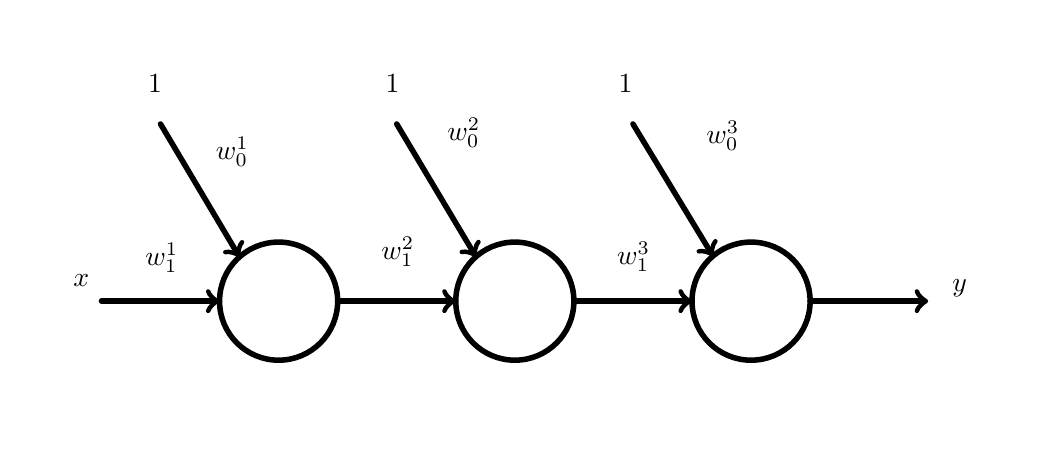
\begin{tikzpicture}[scale = 1.5, line cap=round,line join=round,x=1.0cm,y=1.0cm]
		\clip(-4.624679143882289,1.3686903642723092) rectangle (3.8521836267384844,4.8154607149701345);
		\draw [line width=2.pt] (-2.5,2.5) circle (0.5cm);
		\draw [line width=2.pt] (-0.5,2.5) circle (0.5cm);
		\draw [line width=2.pt] (1.5,2.5) circle (0.5cm);
		\draw [->,line width=2.pt] (-3.5,4.) -- (-2.831496141146421,2.874313115459547);
		\draw [->,line width=2.pt] (-4.,2.5) -- (-3.,2.5);
		\draw [->,line width=2.pt] (-2.,2.5) -- (-1.,2.5);
		\draw [->,line width=2.pt] (0.,2.5) -- (1.,2.5);
		\draw [->,line width=2.pt] (2.,2.5) -- (3.,2.5);
		\draw [->,line width=2.pt] (-1.5,4.) -- (-0.8294354120380936,2.8761280490674572);
		\draw [->,line width=2.pt] (0.5,4.) -- (1.1775032003746246,2.8820939861230355);
		\draw (-3.686865302879703,4.5) node[anchor=north west] {$1$};
		\draw (-1.67726421501702,4.5) node[anchor=north west] {$1$};
		\draw (0.2957986712481599,4.5) node[anchor=north west] {$1$};
		\draw (-4.320194130569761,2.805859627107445) node[anchor=north west] {$x$};
		\draw (3.1214195947884176,2.7693214255099416) node[anchor=north west] {$y$};
		\draw (-3.7112241039447054,3.07380643882247) node[anchor=north west] {$w_1^1$};
		\draw (-3.114433477852151,3.9750820782275555) node[anchor=north west] {$w_0^1$};
		\draw (-1.7138024166145234,3.122524040952475) node[anchor=north west] {$w_1^2$};
		\draw (-1.1535499921194723,4.13341428515007) node[anchor=north west] {$w_0^2$};
		\draw (1.0387421037307276,4.109055484085068) node[anchor=north west] {$w_0^3$};
		\draw (0.2836192707156588,3.0859858393549713) node[anchor=north west] {$w_1^3$};
		\end{tikzpicture}
	\end{center} 
	
	В качестве функции активации Маша использовала сигмоиду: $f(t) = \frac{e^t}{1 + e^t}$.  Как это обычно бывает, Маша обнаружила её в своих штанах после стирки и очень обрадовалась. Теперь она хочет сделать два шага стохастического градиентного спуска, используя алгоритм обратного распространения ошибки.
	
	У неё есть два наблюдения: $x_1 = 1, x_2 = 5$, $y_1 =1$, $y_2 = 0$. Скорость обучения $\gamma = 1$. В качестве инициализации взяты нулевые веса. Сначала берётся второе наблюдение, затем первое. Помогите Маше. 
\end{problem}

%%%-------------------------------------------
\begin{problem}{(незаметный backpropagation)}
    
    Маша собрала нейросеть: 
	
	\begin{equation*}
	y =   \max \left( 0;  X \cdot  \begin{pmatrix} 1 & -1 \\ 0.5 & 0 \end{pmatrix} \right) \cdot \begin{pmatrix} 0.5 \\ 1 \end{pmatrix} 
	\end{equation*}

	Теперь Маша внимательно смотрит на неё.
	
	\begin{enumerate}
		\item  Первый слой нашей нейросетки --- линейный. По какой формуле делается forward pass? Предположим, что на вход пришло наблюдение $x = (1, 2)$. Сделайте через этот слой forward pass и найдите выход из слоя.
		
		\item Найдите для первого слоя производную выхода по входу. При обратном движении по нейросетке, в первый слой пришёл накопленный градиент $(-1, 0)$. Каким будет новое накопленное значение градиента, которое выплюнет из себя линейный слой? По какой формуле делается backward pass? 
		
		\item Второй слой нейросетки ---- функция активации, $ReLU.$  По какой формуле делается forward pass? На вход в него поступило значение $(2, -1)$. Сделайте через него forward pass. 
		
		\item Найдите для второго слоя производную выхода по входу. При обратном движении по нейросетке во второй слой пришёл накопленный градиент $(-1, -2)$.  Каким будет новое накопленное значение градиента, которое выплюнет из себя $ReLU$?  По какой формуле делается backward pass? 
		
		\item Третий слой нейросетки --- линейный.  По какой формуле делается forward pass? Пусть на вход поступило значение $(2,0)$.  Сделайте через него forward pass. 
		
		\item Найдите для третьего слоя производную выхода по входу. При обратном движении по нейросетке, в третий слой пришёл накопленный градиент $-2$. Каким будет новое накопленное значение градиента, которое выплюнет из себя линейный слой?  По какой формуле делается backward pass? 
		\item Мы решаем задачу Регрессии. В качестве функции ошибки мы используем $MSE$. Пусть для рассматриваемого наблюдения реальное значение $y = 0$. Найдите значение $MSE$. Чему равна производная $MSE$ по входу (прогнозу)? Каким будет накопленное значение градиента, которое $MSE$ выплюнет из себя в предыдущий слой нейросетки, если изначально значение градиента инициализировано единицей? 
		
		\item Пусть скорость обучения $\gamma = 1$.  Сделайте для весов нейросети шаг градиентного спуска. 
	\end{enumerate}

	Посидела Маша, посидела, и поняла, что неправильно она всё делает. В реальности перед ней не задача регрессии, а задача классификации. 
	
	\begin{enumerate}	
		\item Маша навинтила поверх второго линейного слоя сигмоиду. Как будет для неё выглядеть forward pass? Сделайте его. Найдите для сигмоиды производную выхода по входу.
		
		\item В качестве функции потерь Маша использует $\logloss.$ Как для этой функции потерь выглядит forward pass? Сделайте его. Найдите для $\logloss$ производную выхода по входу. 
		
		\item Как будет выглядеть backward pass через $logloss$ и сигмоиду? Прделайте его. Как изменится процедура градиентного спуска для остальной части сети? 
	\end{enumerate}
\end{problem} 


%%%-------------------------------------------
\begin{problem}{(Ещё один backpropagation)}

    \todo[inline]{Может усложнить задачу?}

	Пусть у нас есть нейронка: 
	
	$$ 
	y = f(X \cdot W_2 ) \cdot W_1 
	$$
	
	Как для функции потерь $L(W_1, W_2) = (y - \hat y)^2$ будет выглядеть алгоритм обратного распространения ошибки, если $f(t) = ReLU(t) =  \max(0; t)$? Найдите все выходы, все промежуточные производные.  Опишите правило, по которому производная будет накапливаться, а также сам шаг градиентного спуска. 
\end{problem} 

\todo[inline]{Какую-нибудь задачу про Нестерова в бэкпропе по мотивам вопроса с пары про то как правильно обновлять веса}
